\hypertarget{different-code-metric-tools}{%
\section{Different Code-Metric
Tools}\label{different-code-metric-tools}}
We differentiate between Static Code Analyzer which analyses the code in the IDE whereas Repository Analyzers analyse the statistics of the repository. Those tools provide a rough overview of the legacy or the actual code. They should be used frequently to compare the numbers. Those numbers determine the quality of the code in terms of their metrics.



\hypertarget{Code Metrics}{%
\subsection{Code Metrics}\label{Code-Metrics}}
\begin{figure}[H]
\centering
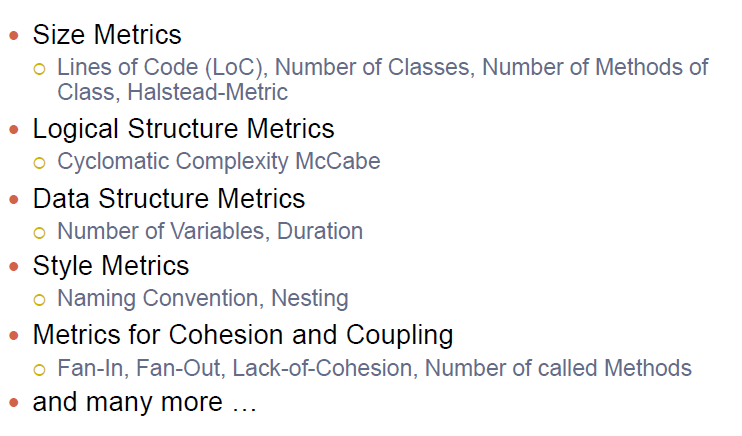
\includegraphics[width=0.5\textwidth]{figures/CodeMetrics.png}
\caption{Code Metrics}
\end{figure}




\hypertarget{gource}{%
\subsection{Gource}\label{gource}}

\begin{itemize}
\tightlist
\item
  Software projects can be displayed as an animated tree
\item
  Directories appear as branches while files are their leaves
\item
  Develpers ca nbe seen working on the tree they contributed to
\end{itemize}

\hypertarget{code-city}{%
\subsection{Code City}\label{code-city}}

\begin{itemize}
\tightlist
\item
  Standalone or as plugin for eclipse
\item
  Needs a lot of knowledge and pre-work to get it running
\item
  It shows the code as a city

  \begin{itemize}
  \tightlist
  \item
    The packages are parcels of land
  \item
    classes are shown as buildings
  \end{itemize}
\end{itemize}

\hypertarget{pros}{%
\subsubsection{Pros}\label{pros}}

\begin{itemize}
\tightlist
\item
  Very good overview for large code bases
\item
  Fast identification of oversized classes in terms of lines of code and
  amount of methods
\end{itemize}

\hypertarget{cons}{%
\subsubsection{Cons}\label{cons}}

\begin{itemize}
\tightlist
\item
  Intermediate MSE format
\item
  The software is not stable
\item
  Small community
\item
  Development is inactive since 2009
\end{itemize}



\subsection{More Tools}
\subsubsection{Static Code Analyzer}
\begin{itemize}
    \item Code City
    \item Sonargraph
    \item SonarQube
\end{itemize}


\subsubsection{Repository Analyzer}
\begin{itemize}
    \item Gource
    \item GitStat
    \item CodeScene
\end{itemize}


\hypertarget{Polymetric View}{%
\subsection{Polymetric View}\label{Polymetric-View}}
\begin{figure}[H]
\centering
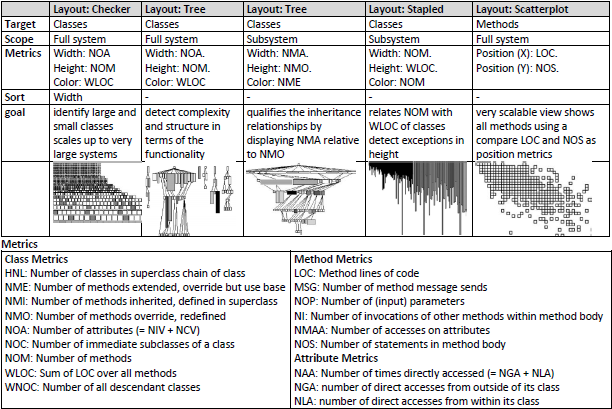
\includegraphics[width=0.5\textwidth]{figures/Polymetric.PNG}
\caption{Polymetric View}
\end{figure}
\clearpage

